\section{Theoretical foundations}
\label{sec:Theorie}
\subsection{The FACT telescope}
The \textit{First G-APD Cherenkov Telescope} (FACT) is a cherenkov telescope operating in the Observatorio del Roque de los Muchachos located in La Palma, Spain since 2011.
Its purpose is to observe the brightest sources of gamma radiation.
FACT mainly observes the crab nebula, a super nova remnant in the milky way, as well as extra galactic blazars.
FACT has been remote-controlled since 2012 and has been operating automatically since 2017.
A picture of the FACT telescope can be found in figure \ref{fig:FACT}

\begin{figure}
  \centering
  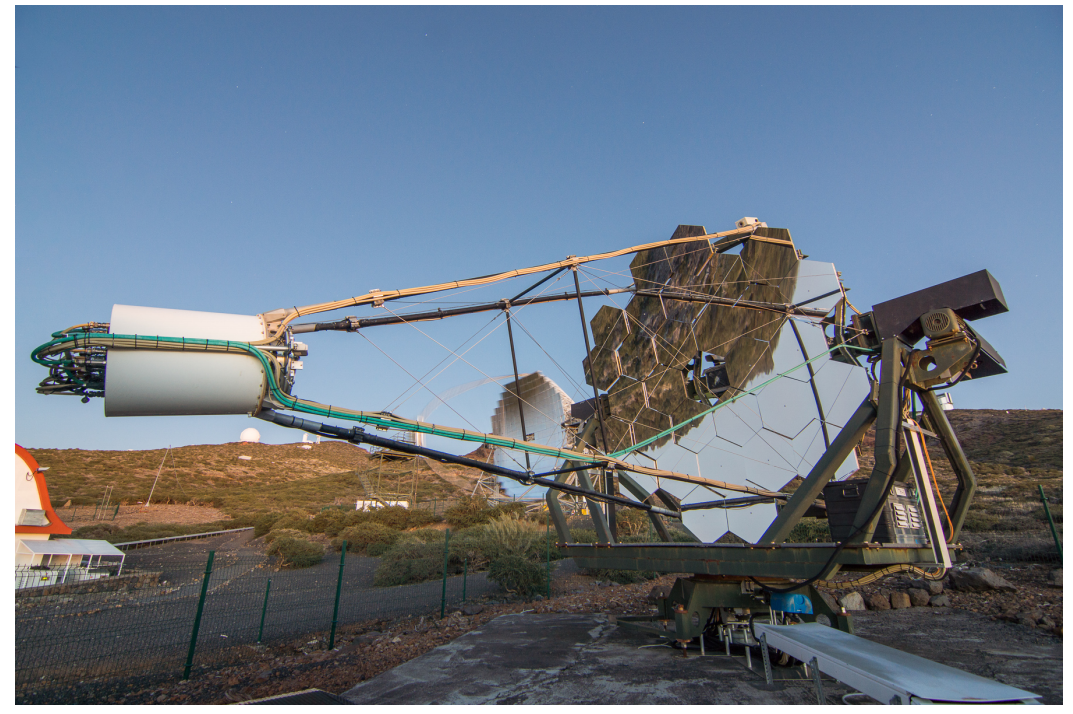
\includegraphics[width=0.7\textwidth]{graphics/FACT.png}
  \caption{A picture of FACT at the Observatorio del Roque de los Muchachos, La Palma, Spain \cite{sample}.}
  \label{fig:FACT}
\end{figure}

To measure the observed sources at the same time as estimating the background rate FACT uses the so called Wobble mode.
For that the telescope measures data from $\SI{0.6}{\degree}$ next to the source.
Next to the source geometric equivalent points (off positions) can be defined which only contain background while the source itself contains the wanted data (on position).
Figure \ref{fig:OnOff} shows the on position and the off position.

\begin{figure}
  \centering
  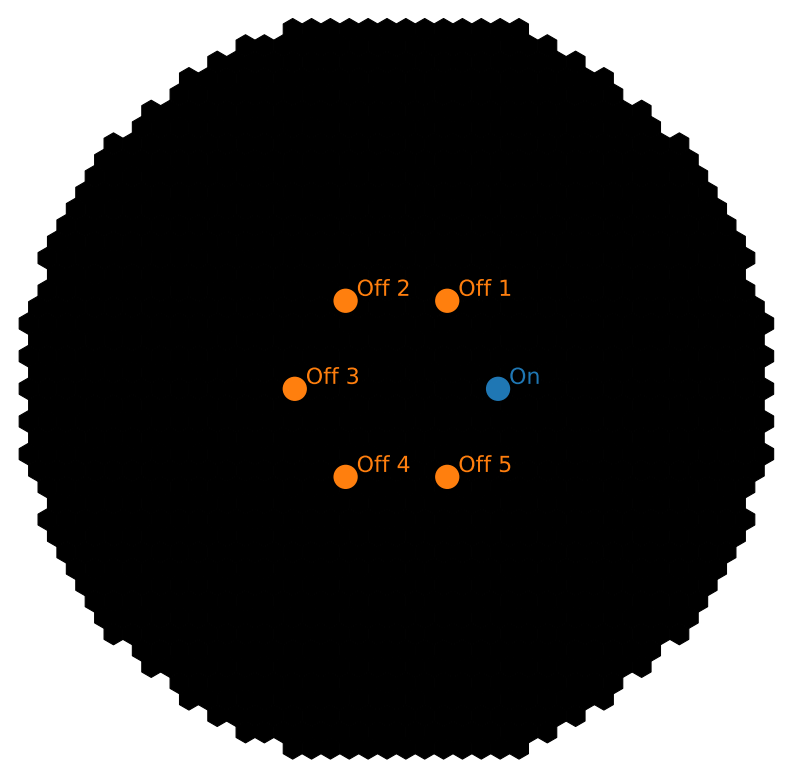
\includegraphics[width=0.5\textwidth]{graphics/OnOff.png}
  \caption{FACT camera picture with on position and 5 off positions \cite{sample}.}
  \label{fig:OnOff}
\end{figure}

Events taken from the on region are labeled as $N_{on}$ while events from the off region are labeled as $N_{off}$.
This results to a detector significance of
\begin{equation*}
  \symup{S} = \sqrt{2}\cdot \sqrt{N_{on} \ln\left( \frac{1 + \alpha}{\alpha} \left(  \frac{N_{on}}{N_{on} + N_{off}}\right)\right) + N_{off} \ln\left( (1 + \alpha) \left(\frac{N_{off}}{N_{on} + N_{off}}\right)\right)} \, ,
\end{equation*}
where $\alpha$ is ratio of the on-region and off-region.
With 5 off regions in this Wobble mode $\alpha$ is equal to $0.2$.

\subsection{Data Sets}
The given data sets have already been prepared.
The following steps have been done to produce the given data.
For every shower event three attributes have to be reconstructed: particle class, energy and direction of origin.
To determine these complex simulations are needed to create the training data sets.
Air shower and cherenkov production as well as particle propagation are simulated by the software \texttt{CORSIKA}.
After saving the simulated light that arrives at the telescope the software \texttt{CERES} is used to simulate the detector and all its components.
The simulated data is created in a way that it has the same format as the real data that was measured by the telescope.
Three data sets have been simulated for this analysis:
\begin{itemize}
  \item gammas from point-like source, observed with wobble mode
  \item gammas coming from random directions
  \item protons coming from random directions
\end{itemize}

\subsection{Unfolding}
In astrophysical measurements the parameters of interests are mostly measured indirectly.
The measured energy deposits and measured parameters are usually used to determine the attributes of the particles of interest.
This so called "inverse problem" can be described by the equation
\begin{equation}
  g(y) = \int A(y,x) f(x) \symup{d}x + b(y) \,.
  \label{eqn:convo}
\end{equation}

Here $f(x)$ describes the probability density function of interest, depending on the physical parameter x.
The background is described by $b(y)$ where $y$ is the measured parameter.
The probability density function of the measured parameter is given by $g(y)$ and $A(y,x)$ is the convolution core describing the detector.
Unfolding techniques are used to solve this problem.
Discretizing \eqref{eqn:convo} gives the form
\begin{equation}
  \symbf{g} = \symbf{A}\symbf{f} + \symbf{b} \, .
\end{equation}
Here $g$ is the histogram of estimated gamma-energies, $A$ is a smearing matrix representing the stochastic process happening in the detector and distorting the true values, $f$ is the histogram of the true gamma-energies and $b$ is the background from the off positions.

\subsubsection{Naive SVD Unfolding}
An easy solution of the unfolding is inverting $A$.
In the case of non-quadratic matrices the Moore-Penrose-Pseudoinverse is being calculated with
\begin{equation}
  \hat{\symbf{f}} = \symbf{A}^{+}(\symbf{g} - \symbf{b}) \, .
  \label{eqn:svd}
\end{equation}
This solution is equivalent to the method of least squares.

\subsubsection{Poisson-Likelihood-Unfolding}
Presuming that $g$ is poisson distributed, a maximum likelihood fit can be done.
The probability to measure $g_i$ is
\begin{align}
  \symup{P}(g_i) &= \mathcal{P}(g_i, \lambda_i) = \frac{\lambda_i^{g_i}}{g_i!}\text{e}^{-\lambda_i} \\
  \shortintertext{with}
  \symbf{\lambda} &= \symbf{A}\symbf{f} + \symbf{b} \\
  \intertext{minimizing the negative log-likelihood yields}
  -\ln(\mathcal{L}) &= \sum_{i=1}^{M} = -g_i \ln(\lambda_i) + \lambda_i \\
  \intertext{the estimator for $\symbf{f}$ is then}
  \hat{\symbf{f}} &= \text{argmin}(-\ln(\mathcal{L}(\symbf{f}|\symbf{A},\symbf{g},\symbf{b})))\, .
\end{align}
